%*****************************************
\chapter{Visualizing Dispersion} \label{vdi:visualizing_dispersion}
%*****************************************
%TODO Reviewed

\section{Introduction}
\texttt{SOFA} makes it easy to calculate various measures of dispersion, as covered in Lab \ref{dis:data_dispersion}; however, most people find it easier to understand the dispersion of data when that is presented graphically. Fortunately, \texttt{SOFA} has a great graphic tool for visualizing data dispersion: Box Plot (sometimes called ``Box and Whisker'' plot). A Box Plot graphically illustrates Q1, the median, Q3, and outliers (if any are present). 

The \textit{bdims} dataset is used to illustrate a Box Plot. Following is the statistical data for \textit{Age} from the \textit{bdims} dataset along with the box plot for that same data.

\rowcolors{1}{gray!25}{}
\begin{center}
  \begin{tabular}{ccccccc}
    \hline 
    \multicolumn{7}{c}{\textbf{Age (years)}} \\ 
    \hline 
    \textbf{Min} & \textbf{Q1} & \textbf{Median} & \textbf{Q3}  & \textbf{Max} & \textbf{Range} & \textbf{IQR} \\ 
    \hline 
    $ 18 $ & $ 23 $ & $ 27 $ & $ 36 $ & $ 67 $ & $ 49 $ & $ 13 $ \\ 
    \hline 
  \end{tabular} 
\end{center}

Following is the box plot that illustrates the above statistics.

\begin{figure}[H]
  \begin{center}
    \fbox{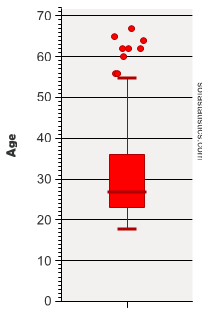
\includegraphics[width=0.50\linewidth]{gfx/vdi005}}
    \caption{Box Plot for Bdims Age}
  \end{center}
\end{figure}

In the above Box Plot, the median is indicated by a dark line at $ 27 $, Q1 is $ 23 $ (the lower edge of the box) and Q3 is $ 36 $ (the upper edge of the box). That makes the Inter-Quartile Range (IQR) equal to $ 13 $ (the size of the box). 

The ``whiskers'' are placed at $ 1.5 X IQR $ above and below each quadrant. Thus:

\begin{enumerate}
  \item \textbf{Upper}. $ Q3  + ( 1.5 X IQR $), or $ 36 $ + ($ 1.5 X 13 $) = $ 55.5 $
  \item \textbf{Lower}. $ Q1  – ( 1.5 X IQR $), or $ 23 $ – ($ 1.5 X 13 $) = $ 19.5 $
\end{enumerate}

Note: \texttt{SOFA} makes it possible to set the whiskers at the maximum and minimum values, but that hides the outliers and is rarely done.

The circles above the box plot represent outliers. In this case there are nine outliers. If the data are a normal distribution, then the whiskers will enclose most of the values in the dataset and outliers will be rare.

Here is a second example from the same dataset:

\rowcolors{1}{gray!25}{}
\begin{center}
  \begin{tabular}{ccccccc}
    \hline 
    \multicolumn{7}{c}{\textbf{Height (cm)}} \\ 
    \hline 
    \textbf{Min} & \textbf{Q1} & \textbf{Median} & \textbf{Q3}  & \textbf{Max} & \textbf{Range} & \textbf{IQR} \\ 
    \hline 
    $ 147.20 $ & $ 163.80 $ & $ 170.30 $ & $ 177.80 $ & $ 198.10 $ & $ 50.90 $ & $ 14.00 $ \\ 
    \hline 
  \end{tabular} 
\end{center}

\begin{figure}[H]
  \begin{center}
    \fbox{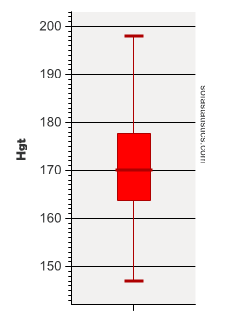
\includegraphics[width=0.50\linewidth]{gfx/vdi010}}
    \caption{Box Plot for Bdims Height}
  \end{center}
\end{figure}

In this case, there are no outliers so there are no circles above or below the whiskers. Also, the data are very ``bunched up'' and all values lie inside $ 1.5 $ times the minimum and maximum values, so the whiskers lie at the minimum and maximum.

Box plots become much more useful when more than one data item is plotted side-by-side for comparison. For example, the following box plot is helpful in determining if there is a difference in height by sex.

\begin{figure}[H]
  \begin{center}
    \fbox{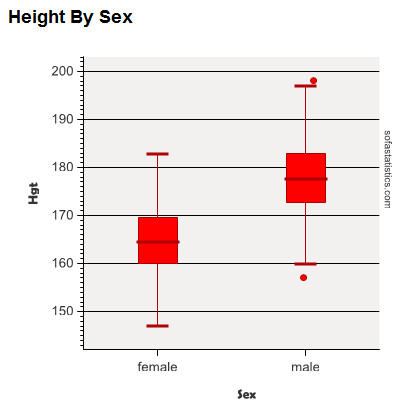
\includegraphics[width=0.75\linewidth]{gfx/vdi015}}
    \caption{Comparing Height By Sex}
  \end{center}
\end{figure}

By comparing the two box plots it is very easy to see that males are generally taller than females since that box is higher on the graph. Also notice that the ``males'' plot includes outliers at both the minimum and maximum values which indicates a greater variation in male heights than female.

As a final example of box plots, consider the \textit{cars} dataset. The following box plot shows the price of a new automobile by the number of passengers it can carry.

\begin{figure}[H]
  \begin{center}
    \fbox{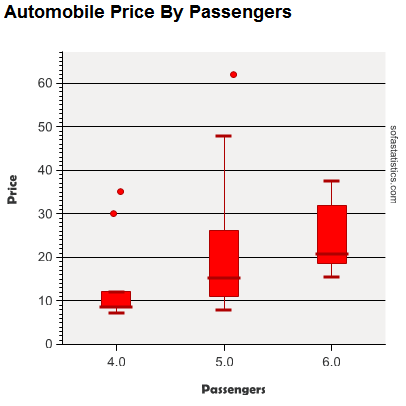
\includegraphics[width=\linewidth]{gfx/vdi020}}
    \caption{Car Prices By Passenger Capacity}
    \label{vdi:img04}
  \end{center}
\end{figure}

An analysis of Figure \ref{vdi:img04} leads to the following:

\begin{itemize}
    \item Generally, four-passenger cars are less expensive than five-passenger cars and they, in turn, are less expensive than six-passenger cars since the boxes for those vehicles are progressively higher on the graph.
    \item Five-passenger automobiles have a wider spread of prices than the other two types. 
    \item Notice that for five-passenger automobiles the upper whisker is a long way from the top of the box. That indicates that the dataset are skewed such that most values are between about \$$ 12 $K and \$$ 27 $K but there are a number of values that are higher along with one outlier above \$$ 60 $K.
    \item The box for the four-passenger cars is small and the whiskers are nearly the same as the ends of the box which means that there is very little variation in the prices, though there are two extreme outliers.
\end{itemize}

\section{Procedure}

\subsection{Boxplots}

Start \texttt{SOFA} and select ``Charts.'' Then:

\begin{enumerate}
  \item Data Source Table: births
  \item Chart Types: Make Box and Whisker Plot (the last button on the right)
  \item Variables Described: Gained (gained)
  \item Title: Weight Gained
\end{enumerate}

\begin{figure}[H]
  \begin{center}
    \fbox{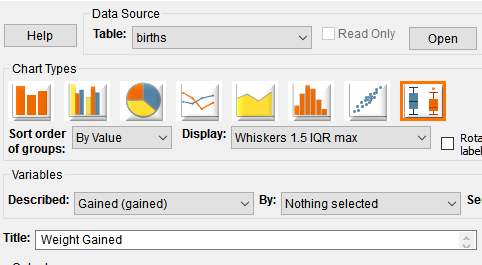
\includegraphics[width=\linewidth]{gfx/vdi025}}
    \caption{Set Up Boxplot for Weight Gained}
  \end{center}
\end{figure}

Following is the plot generated by the above.

\begin{figure}[H]
  \begin{center}
    \fbox{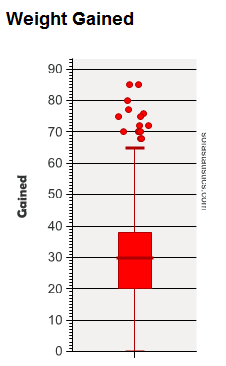
\includegraphics[width=0.5\linewidth]{gfx/vdi030}}
    \caption{Box Plot of Weight Gained}
  \end{center}
\end{figure}

\subsection{Activity 1: Simple Boxplot} \label{vdi:act01}

Using the \textit{maincafe} dataset in \texttt{SOFA}, produce a boxplot for Age. The boxplot should have a title of ``Visualizing Dispersion, Activity 1'' and a subtitle of ``Boxplot For Age''.

\subsection{Grouped Boxplot}

To group two or more boxplots, select a grouping variable to create grouped plots. For example, to group the weight gain box plots by whether the mother was a smoker, select:

\begin{enumerate}
  \item Data Source Table: births
  \item Chart Types: Make Box and Whisker Plot (the last button on the right)
  \item Variables Described: Gained
  \item By: Habit
  \item Title: Weight Gained by Smoking Habit
\end{enumerate}

\begin{figure}[H]
  \begin{center}
    \fbox{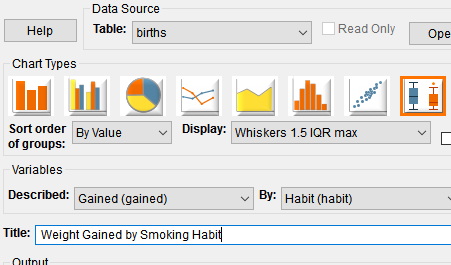
\includegraphics[width=\linewidth]{gfx/vdi035}}
    \caption{Set Up Boxplot for Weight Gained by Habit}
  \end{center}
\end{figure}

\begin{figure}[H]
  \begin{center}
    \fbox{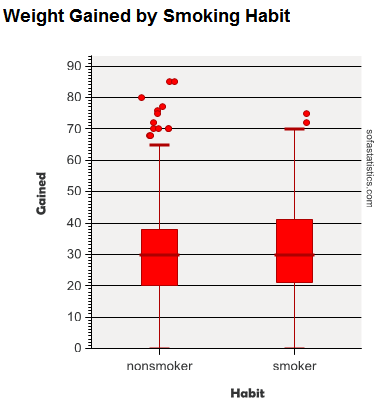
\includegraphics[width=0.8\linewidth]{gfx/vdi040}}
    \caption{Box Plot of Weight Gained by Habit}
  \end{center}
\end{figure}

\subsection{Activity 2: Grouped Boxplots} \label{vdi:act02}

Using the \textit{maincafe} dataset in \texttt{SOFA}, produce a boxplot for Age grouped by Meal. The boxplot should have a title of ``Visualizing Dispersion, Activity 2'' and a subtitle of ``Boxplot of Age Grouped By Meal''.

\subsection{Grouped Boxplots By Series}

Finally, the data can be grouped by series. For example, to group the above box plots by the sex of the baby, select ``Gender'' as the ``Series By'' variable and then change the title and subtitle of the box plot. 

\begin{figure}[H]
  \begin{center}
    \fbox{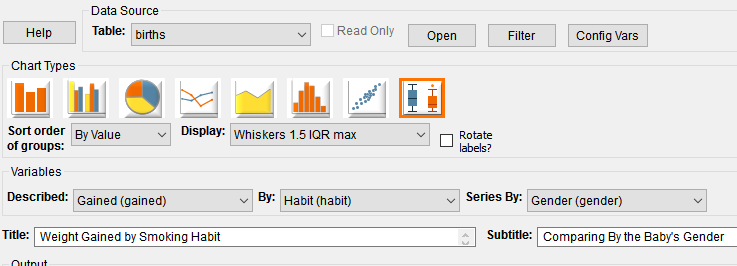
\includegraphics[width=\linewidth]{gfx/vdi045}}
    \caption{Set Up Boxplot for Weight Gained by Habit and Baby's Sex}
  \end{center}
\end{figure}

\begin{figure}[H]
  \begin{center}
    \fbox{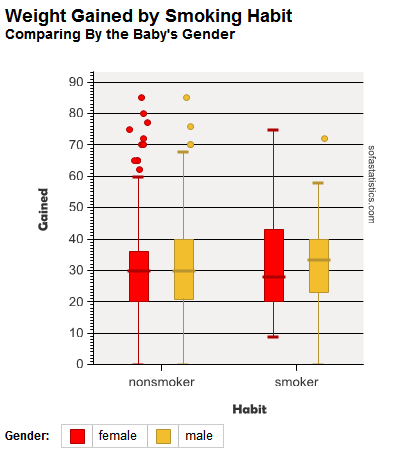
\includegraphics[width=0.8\linewidth]{gfx/vdi050}}
    \caption{Box Plot of Weight Gained by Habit and Baby's Sex}
    \label{vdi:img10}
  \end{center}
\end{figure}

In box plot \ref{vdi:img10} it is clear that for non-smokers, male baby's weights are more variable than females since that box is larger. Interestingly, the weight of female babies born to smokers has a much larger variability (the box is larger) and the mean of the weights for female babies is somewhat lower than for males.

As a second example of a box plot, the \textit{email} dataset was selected and the size of the email message (number of characters) was plotted as a function of whether it was spam and contains large numbers. 

\begin{figure}[H]
  \begin{center}
    \fbox{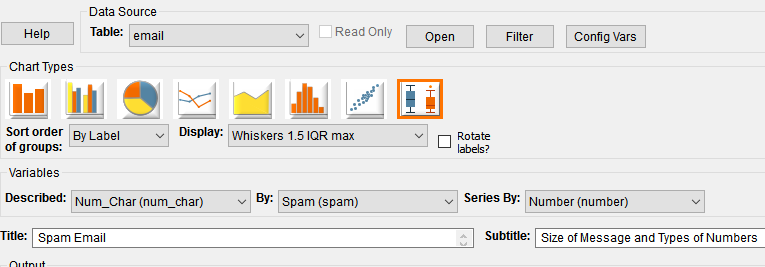
\includegraphics[width=\linewidth]{gfx/vdi055}}
    \caption{Set Up Boxplot for Email Data Set}
  \end{center}
\end{figure}

\begin{figure}[H]
  \begin{center}
    \fbox{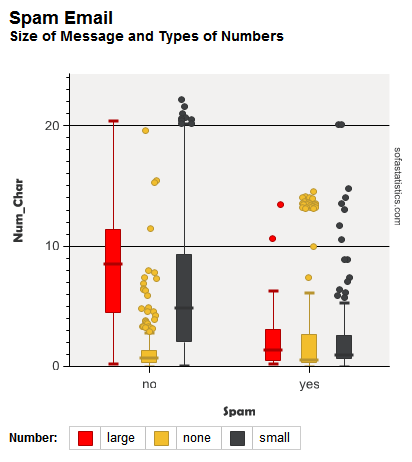
\includegraphics[width=0.8\linewidth]{gfx/vdi060}}
    \caption{Example Box Plot for Email Data Set}
    \label{vdi:img12}
  \end{center}
\end{figure}

To interpret box plot \ref{vdi:img12}, notice that, generally, the spam messages contain fewer characters than non-spam messages (those plots are lower), indicating that spam messages are generally shorter than non-spam messages. Then, looking at only the non-spam plots (the three on the left), notice that if the message contains large numbers (the first plot from the left) it will generally contain more characters than messages with only small numbers (the third plot). Finally, notice that non-spam messages with no numbers (the second plot) are generally short (fewer characters, indicated by a box that is lower on the scale). There are a number of other characteristics that could be drawn from this one chart, such as a discussion about the outliers or the means for each type of message.

The last example (the email box plots) illustrates that a box plot contains a lot of information and is a valuable tool for research reports. 

\subsection{Activity 3: Grouped Boxplots by Series} \label{vdi:act03}

Using the \textit{maincafe} dataset in \texttt{SOFA}, produce a boxplot for Age grouped by Sex and using Meal as a series. The boxplot should have a title of ``Visualizing Dispersion, Activity 3'' and a subtitle of ``Boxplot of Age by Sex and Meal''.

\section{Deliverable}

Complete the following activities in this lab:

\rowcolors{1}{gray!25}{}
\begin{center}
  \begin{tabular}{lll}
    \hline 
    \textbf{Number} & \textbf{Name} & \textbf{Page} \\ 
    \hline 
    \ref{vdi:act01} & \nameref{vdi:act01} & \pageref{vdi:act01} \\ 
    \ref{vdi:act02} & \nameref{vdi:act02} & \pageref{vdi:act02} \\ 
    \ref{vdi:act03} & \nameref{vdi:act03} & \pageref{vdi:act03} \\ 
    \hline 
  \end{tabular} 
\end{center}

Consolidate the responses for all activities into a single document and submit that document for grading.
